\part{Degrees of Freedom and Phases}
\section{The Phase Rule}
\subsection{Phase}
\begin{definition}
    \textbf{Phase}, p, is a state of matter that is \textbf{uniform}\mn{ When we talk about uniform, specified length and time scales are needed. If there are no specifications of these scales, the meaning of uniform itself becomes unclear. Usually, the specification is related to the problem we are discussing about.} throughout in both chemical composition and physical states.
\end{definition}
\paragraph{Phase numbers of common forms of matters}~\\~\\
\begin{threeparttable}
    \begin{tabular}{cc}
        \toprule
        form of matter & number of phases\\
        \midrule
        gas & p=1\\
        solution & p=1\\
        liquid & canbe multiple phases\\
        solid\tnote{*} & each solid of different chemical composition\mn{When the length scale of the system decreases into mesoscale, the chemical composition is hard to clearify and becomes very complex. So traditional phase theory can be hard to use in nano science.} is in one phases\\
        \bottomrule
    \end{tabular}
    \begin{tablenotes}
        \footnotesize
        \item[*] One solid phase can contain different substances, e.g. steel, and in general, for allays, $p=1$ (but p may greater than 1 in some cases.
    \end{tablenotes}
\end{threeparttable}
\subsection{Constituent and Components}
\begin{definition}
    \textbf{Constituent} is a chemical species present.
\end{definition}
\begin{definition}
    \textbf{Component}, c, is \emph{independent} constiuent present.
\end{definition}
\begin{example}
    To explain the meaning of \emph{independent contituents}, some examples are provided below.\\
    \begin{itemize}
        \item $\ce{CaCO3(s) <=> CaO(s) + CO2(g)}$\\
        The number of constiuents in the system is obviously 3. However, an reaction relates the three constituents, therefore, the number of components in the system is 2.
        \item $\ce{NH4Cl(s) <=> NH3(g) + HCl(g)}$\\
        If no additional $\ce{NH3}$ or $\ce{HCl}$ is added to the system, $c=3-1-1=1$. For except a restrain from the chemical reaction, there is another equation: $n(\ce{NH3})=n(\ce{HCl})$. And if additional $\ce{NH3}$ or $\ce{HCl}$ is added, $c=2$.
        \item $\ce{H2O}, \ce{H2} \text{ and } \ce{O2}$\\
        $c$ can be $1, 2$ or $3$. Although when the system is in equilibrium, $c=3$ is impossible, under most conditions (e.g. 1 \si{bar} and room temperature), in the time sclae we considering, the equilibrium is har to reach. And under these circumstances, $c=3$ is possible to occur.
    \end{itemize}
\end{example}
\subsection{Degrees of freedom}
\begin{definition}
    The \textbf{degree of freedom}, $F$, is the number of \emph{intensive variables} that can be changed \emph{independently} without disturbing the phase of the system.
\end{definition}
\begin{example}
    Some examples are given to show the identification of $F$.\\
    \begin{itemize}
        \item pure liquid water\\
        For pure liquid water, the system itself can be explained by 4 variables, $T, p, V, n$, in which $n$ is not an intensive variable and therefore can be ignored. The other three vars are restrained by the state equation, which gives out the result that for pure liquid water system, $F=2$.
        \item mixture of liquid water and steam\\
        The situation is similar to the example above, but there is another restrain function that $\mu(\text{g})=\mu(\text{s})$. So $F=1$.
        \item mixture of water, steam and ice\\
        Trivially $F=0$.
        \item mixture of water and methanol\\
        Other than $T, p, V$, $x_1$ is also intensive variable\mn{$x_2$ is not independent for $x_1+x_2=1$}. Two restrains exists, including the state equation and the equilibrium of chemical potential. Thus $F=2$.
    \end{itemize}
\end{example}
\subsection{The phase rule}
\begin{theorem}[Phase rule]
    In thermodynamics, the \textbf{phase rule} is a general principle governing "pVT" systems (that is, systems whose states are completely described by the variables pressure ($p$), volume ($V$) and temperature ($T$)) in thermodynamic equilibrium. If $F$ is the number of degrees of freedom, $C$ is the number of components and $P$ is the number of phases, then:
    \begin{equation}
        F=C-P+2
    \end{equation}
\end{theorem}
\begin{proof}
    The Gibb’s phase rule on the basis of the thermodynamic rule can be derived as follows:
    
    First, let us consider a heterogeneous system consisting of $P_n$ number of phases and $C_n$ number of components in equilibrium. Let us assume that the passage of a component from one phase to another doesn’t involve any chemical reaction. When the system is in equilibrium, it can be described by the following parameters:
    \begin{itemize}
        \item Temperature
        \item Pressure
        \item The composition of each phase
    \end{itemize}

    The total number of variables required to specify the state of the system is:
    \begin{itemize}
        \item Pressure: same for all phases
        \item Temperature: same for all phases
        \item Concentration
    \end{itemize}

    The independent concentration variables for one phase with respect to the $C$ components is $C-1$. Therefore, the independent concentration variables for $P$ phases with respect to  $C$ components is $P(C-1)$, thus the total number of variables is 
    
    $$P(C-1)+2$$
    
    The various phases present in the system can only remain in equilibrium when the chemical potential ($\mu$) of each of the component is the same in all phases. The number of equilibria for each $P$ phases for each component is $P-1$. For $C$ components, the number of equilibria for $P$ phases is $P(C-1)$. Hence, the total number of equilibria involved is 
    
    $$C (P-1)$$

    Therefore,
    $$F=[P(C-1)+2]-C(P-1)=C-P+2$$
\end{proof}
\section{The phase diagrams}
\subsection{Vapour pressure diagram}
The partial vapour pressures of the components of an ideal solution of two volatile liquids are related to the composition of the liquid mixture by Raoult's law
\begin{align}
    \begin{split}\notag
        p_A=x_ap_A^*\quad p_B=x_Bp_B^*
    \end{split}
\end{align}
where $p_A^*$ and $p_B^*$ are vapour pressures of pure A and B. The total vapour pressure p of the mixture is therefore
$$p=x_Ap_A^*+x_Bp_B^*=p_B^*+(p_A^*-p_B^*)x_A$$
\subsubsection{The composition of the vapour}
We define the fraction of A in the gas phase as $y_A$, similarly, $y_B$ is the fraction of B in the vapour. Obviously,
$$y_i=\frac{p_i}{p}\quad i=A,B$$
It is trivial that
$$y_A=\frac{x_Ap_A^*}{p_B^*+(p_A^*-p_B^*)x_A}\quad y_B=1-y_A$$
Simple derivation give out that
$$p=\frac{p_A^*p_B^*}{p_A^*+y_A(p_B^*-p_A^*)}$$
which can be ploted as below.
\begin{figure}[H]
    \setlength{\abovecaptionskip}{0.5pt}
    \centering
    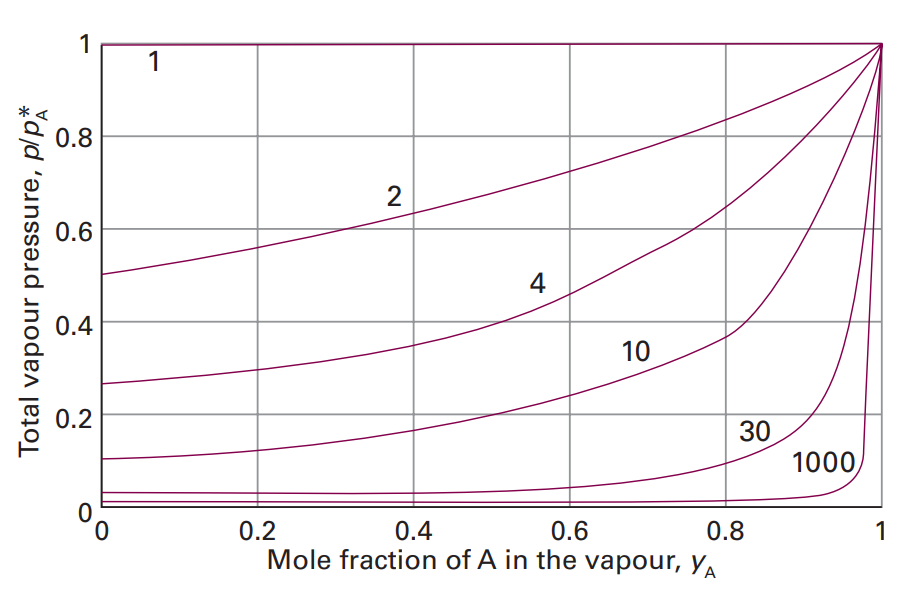
\includegraphics[width=0.6\textwidth]{"./fig/f1.png"}
    \caption{The dependence of the vapour pressure expressed in terms of the mole 
    fraction of A in the vapour.}
\end{figure}
\subsubsection{The interpretation of the diagrams}
If we are interested in distillation, both the vapour and the liquid compositions are of equal interest. Thus we can plot the dependence of the total vapour pressure of an ideal solution on the mole fraction of A in the entire system. 
\begin{figure}[H]
    \setlength{\abovecaptionskip}{0.5pt}
    \centering
    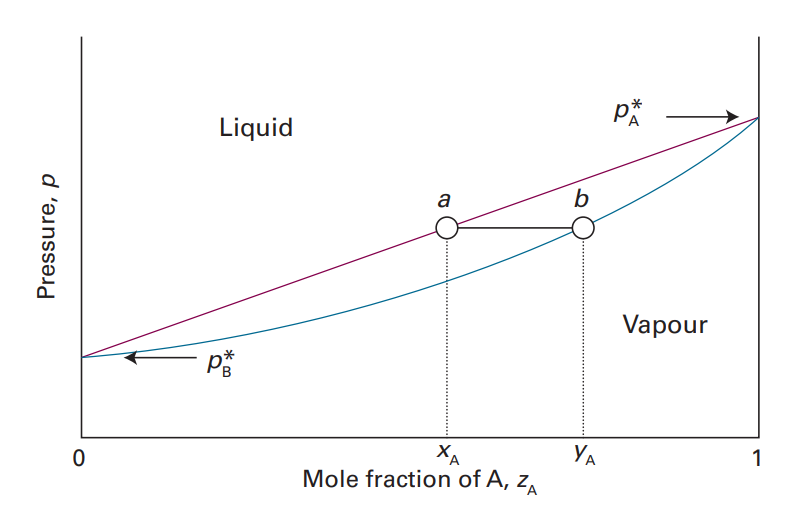
\includegraphics[width=0.6\textwidth]{"./fig/f2.png"}
    \caption{The dependence of the total vapour pressure of an ideal solution on the mole fraction of A in the entire system. }
\end{figure}
In the figure above, $z_A$ is defined as
$$z_A=\frac{n_A(\text{g})+n_A(\text{l})}{n_A+n_B}$$
The point $a$ indicates the vapour pressure of a mixture of composition $x_A$, and the point $b$ indicates the composition of the vapour that is in equilibrium with the liquid at that pressure.

All the points down to the solid diagonal line in the graph correspond to a system that is under such high pressure that it contains only a liquid phase, so $z_A =x_A$, the composition of the liquid. On the other hand, all points below the lower curve correspond to a system that is under such low pressure that it contains only a vapour phase, so $z_A =y_A$.

Points that lie between the two lines correspond to a system in which there are two phases present, one a liquid and the other a vapour.
\subsubsection{The lever rule}
A point in the two-phase region of a phase diagram indicates not only qualitatively that both liquid and vapour are present, but represents quantitatively the relative amounts of each.
The relative amounts of two phases $\alpha$ and $\beta$ can be found by using the lever rule\mn{The lever rule is so called because a similar rule relates the masses at two ends of a lever to their distances from a pivot.}.
\begin{theorem}[lever rule]
    The \textbf{lever rule} can be written as below:
    $$n_\alpha l_\alpha=n_\beta l_\beta$$
    where $n_\alpha$ is the amount of phase $\alpha$ and $n_\beta$ is the amount of $\beta$, $l_\alpha$ and $l_\beta$ represents the distance along the gorizontal line, which is shown in the figure below.
    \begin{figure}[H]
        \setlength{\abovecaptionskip}{0.5pt}
        \centering
        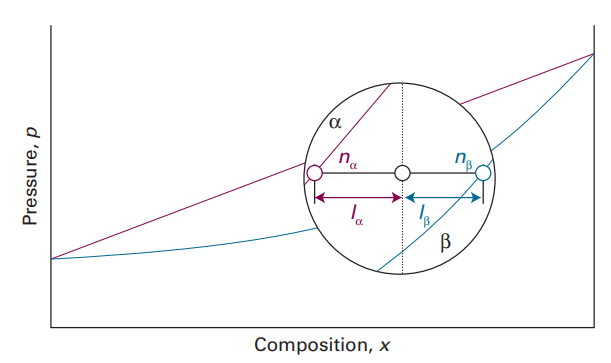
\includegraphics[width=0.6\textwidth]{"./fig/f3.png"}
        \caption{The lever rule}
    \end{figure}
\end{theorem}
\begin{proof}
    The proof of the lever rule is quite trivial. We mark the total amount of A and B as $n=n_\alpha+n_\beta$, where $n_\alpha$ is the amount of phase $\alpha$ and $n_\beta$ is the amount of $\beta$. The mole fraction of A in phase $\alpha$ is $x_{A,\alpha}$, so the amount of A in $\alpha$ is $n_\alpha x_{A,\alpha}$. Similarly, The amount of A in $\beta$ is $n_\beta x_{A,\beta}$, therefore
    $$n_A=n_\alpha x_{A,\alpha}+n_{\beta}x_{A,\beta}$$
    Also, 
    $$n_A=nz_A=n_\alpha z_A+n_\beta z_A$$
    Just equating these two representations will give out the lever rule.
\end{proof}
\subsection{Temperature-composition diagrams}
\begin{marginfigure}
    \setlength{\abovecaptionskip}{0.5pt}
    \centering
    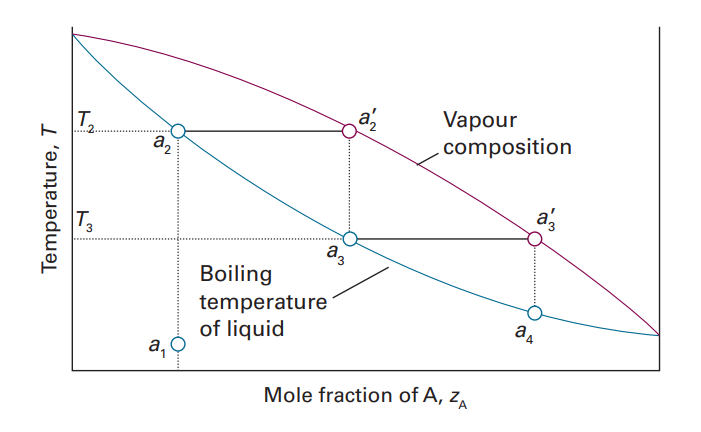
\includegraphics[width=\textwidth]{fig/f4.png}
    \caption{The temperature–composition diagram corresponding to an ideal mixture with the component A more volatile than component B. }
    \label{t-c diagram}
\end{marginfigure}
To discuss distillation we need a temperature–composition diagram, a phase diagram in which the boundaries show the composition of the phases that are in equilibrium at various temperatures. An example is given as Fig. \ref{t-c diagram}.
\subsubsection{Azeotropes}
For real solutions, the temperature–composition diagram is always a little bit more complex than the diagram shown above. A maximum in the phase diagram (Fig. \ref{high-boiling azeotrope}) may occur when the favourable interactions between A and B molecules reduce the vapour pressure of the mixture below the ideal value and so raise its boiling temperature: in effect, the A–B interactions stabilize the liquid. Some examples are $\ce{CHCl3} + \text{propanore}$, $\text{nitric acid} + \ce{H2O}$.
\begin{figure}[H]
    \setlength{\abovecaptionskip}{0.5pt}
    \centering
    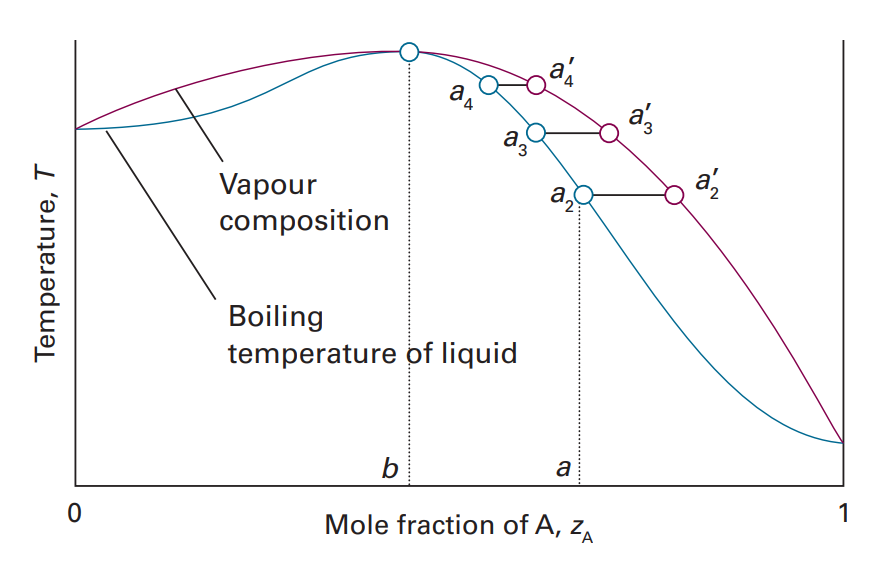
\includegraphics[width=0.6\textwidth]{"./fig/f5.png"}
    \caption{A high-boiling azeotrope.}
    \label{high-boiling azeotrope}
\end{figure}
Phase diagrams showing a minimum (Fig. \ref{low-boiling azeotrope}) indicate that the mixture is destabilized relative to the ideal solution, the A–B interactions then being unfavourable. An example is $\ce{H2O} + \text{ethanol}$.
\begin{figure}[H]
    \setlength{\abovecaptionskip}{0.5pt}
    \centering
    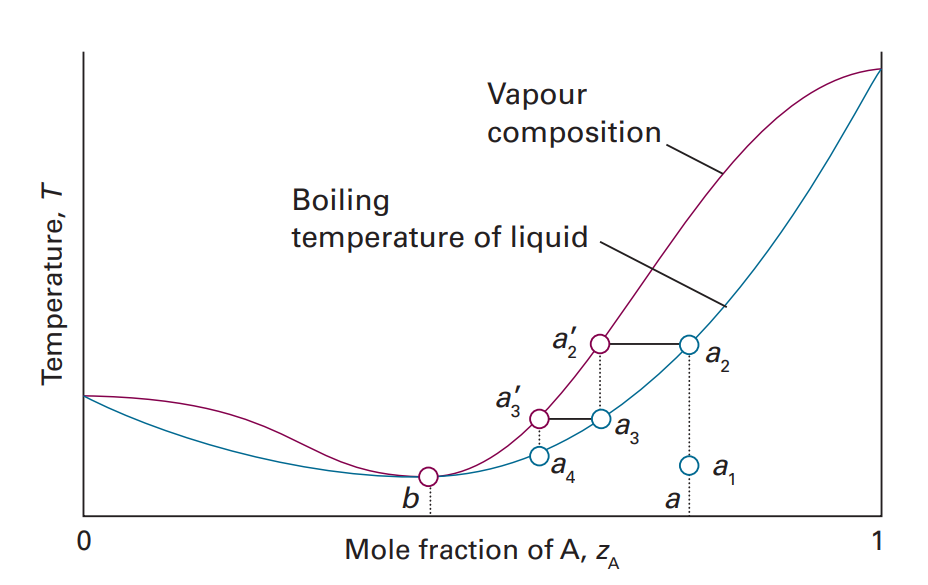
\includegraphics[width=0.6\textwidth]{"./fig/f6.png"}
    \caption{A low-boiling azeotrope.}
    \label{low-boiling azeotrope}
\end{figure}
\begin{definition}
    An \textbf{azeotrope} or a constant boiling point mixture is a mixture of two or more liquids whose proportions cannot be altered or changed by simple distillation. 
\end{definition}
When an azeotrope is boiled, the vapour has the same proportions of constituents as the unboiled mixture. Each azeotrope has a characteristic boiling point. The boiling point of an azeotrope is either less than the boiling point temperatures of any of its constituents (a \textbf{positive azeotrope} or \textbf{low-boiling azeotrope}), or greater than the boiling point of any of its constituents (a \textbf{negative azeotrope} or \textbf{high-boiling azeotrope}).
\subsection{Liquid-liquid phase diagram}





